\documentclass{article}

\usepackage{fancyhdr}
\usepackage{extramarks}
\usepackage{amsmath}
\usepackage{amsthm}
\usepackage{amsfonts}
\usepackage{tikz}
\usepackage[plain]{algorithm}
\usepackage{algpseudocode}
\usepackage{float}
\usepackage{color}
\usepackage{listings}
\usepackage{fontspec}

\setmainfont{BemboStd}
\setmonofont{Menlo}
\newfontfamily\menlo{Menlo}
\lstset{
    columns=fixed,       
    numbers=left,                                        % 在左侧显示行号
    numberstyle=\tiny\color{gray},                       % 设定行号格式
    frame=none,                                          % 不显示背景边框
    backgroundcolor=\color[RGB]{245,245,244},            % 设定背景颜色
    keywordstyle=\color[RGB]{40,40,255},                 % 设定关键字颜色
    numberstyle=\footnotesize\color{darkgray},           
    commentstyle=\small\menlo\color[RGB]{0,96,96},                % 设置代码注释的格式
    stringstyle=\rmfamily\slshape\color[RGB]{128,0,0},   % 设置字符串格式
    showstringspaces=true,                              % 不显示字符串中的空格
    numberstyle=\small\menlo,
    basicstyle=\small\menlo,
    breaklines=true,
}

% \lstset{
%     language=Octave,                % the language of the code
%     basicstyle=\footnotesize,           % the size of the fonts that are used for the code
%     numbers=left,                   % where to put the line-numbers
%     numberstyle=\tiny\color{gray},  % the style that is used for the line-numbers
%     stepnumber=1,                   % the step between two line-numbers. If it's 1, each line 
%                                     % will be numbered
%     numbersep=5pt,                  % how far the line-numbers are from the code
%     backgroundcolor=\color{white},      % choose the background color. You must add \usepackage{color}
%     showspaces=false,               % show spaces adding particular underscores
%     showstringspaces=false,         % underline spaces within strings
%     showtabs=false,                 % show tabs within strings adding particular underscores
%     frame=single,                   % adds a frame around the code
%     rulecolor=\color{black},        % if not set, the frame-color may be changed on line-breaks within not-black text (e.g. commens (green here))
%     tabsize=2,                      % sets default tabsize to 2 spaces
%     captionpos=b,                   % sets the caption-position to bottom
%     breaklines=true,                % sets automatic line breaking
%     breakatwhitespace=false,        % sets if automatic breaks should only happen at whitespace
%     title=\lstname,                 % show the filename of files included with \lstinputlisting;
%                                     % also try caption instead of title
%     keywordstyle=\color{blue},          % keyword style
%     commentstyle=\color{dkgreen},       % comment style
%     stringstyle=\color{mauve},         % string literal style
%     escapeinside={\%*}{*)},            % if you want to add LaTeX within your code
%     morekeywords={*,...}               % if you want to add more keywords to the set
% }

\usetikzlibrary{automata,positioning}

%
% Basic Document Settings
%
%%% page layout
\topmargin=-0.45in
\evensidemargin=0in
\oddsidemargin=0in
\textwidth=6.5in
\textheight=9.0in
\headsep=0.25in

\linespread{1.1}    %%% line spacing

\definecolor{ustcblue}{cmyk}{1,0.8,0,0}

\pagestyle{fancy}
\lhead{\hmwkAuthorName}
\chead{\hmwkClass\ (\hmwkClassInstructor): \hmwkTitle}
\rhead{}
\lfoot{}
\cfoot{\thepage}

\renewcommand\headrulewidth{0.4pt}
\renewcommand\footrulewidth{0.4pt}

\setlength\parindent{0pt}

%
% Create Problem Sections
%

\newcommand{\enterProblemHeader}[1]{
    \nobreak\extramarks{}{Problem \arabic{#1} continued on next page\ldots}\nobreak{}
    \nobreak\extramarks{Problem \arabic{#1} (continued)}{Problem \arabic{#1} continued on next page\ldots}\nobreak{}
}

\newcommand{\exitProblemHeader}[1]{
    \nobreak\extramarks{Problem \arabic{#1} (continued)}{Problem \arabic{#1} continued on next page\ldots}\nobreak{}
    \stepcounter{#1}
    \nobreak\extramarks{Problem \arabic{#1}}{}\nobreak{}
}

\setcounter{secnumdepth}{0}
\newcounter{partCounter}
\newcounter{homeworkProblemCounter}
\setcounter{homeworkProblemCounter}{1}
\nobreak\extramarks{Problem \arabic{homeworkProblemCounter}}{}\nobreak{}

%
% Homework Problem Environment
%
% This environment takes an optional argument. When given, it will adjust the
% problem counter. This is useful for when the problems given for your
% assignment aren't sequential. See the last 3 problems of this template for an
% example.
%
\newenvironment{homeworkProblem}[1][-1]{
    \ifnum#1>0
        \setcounter{homeworkProblemCounter}{#1}
    \fi
    \subsection{Exercise \arabic{homeworkProblemCounter}}
    \setcounter{partCounter}{1}
    \enterProblemHeader{homeworkProblemCounter}
}{
    \exitProblemHeader{homeworkProblemCounter}
}

%
% Homework Details
%   - Title
%   - Due date
%   - Class
%   - Section/Time
%   - Instructor
%   - Author
%

\newcommand{\hmwkTitle}{Homework\ \#5}
\newcommand{\hmwkDueDate}{\today}
\newcommand{\hmwkClass}{Inversion}
\newcommand{\hmwkClassInstructor}{Professor H. Yao \& H. Zhang}
\newcommand{\hmwkAuthorName}{\textbf{Jintao Li}}
\newcommand{\hmwkAuthorID}{\textbf{SA20007037}}
\newcommand{\hmwkAuthoremail}{\textbf{E-mail: lijintao@mail.ustc.edu.cn}}

%
% Title Page
%

% \title{
%     \vspace{2in}
%     \textbf{\hmwkClass:\ \hmwkTitle}\\
%     \normalsize\vspace{0.2in}\large{\hmwkDueDate}\\
%     \vspace{0.2in}\large{\textit{\hmwkClassInstructor}}
%     \vspace{3in}
% }

% \author{\hmwkAuthorName \\
% \hmwkAuthorID}
% \date{}

\renewcommand{\part}[1]{\textbf{ \\ (\alph{partCounter})  }\stepcounter{partCounter} }

%
% Various Helper Commands
%

% Useful for algorithms
\newcommand{\alg}[1]{\textsc{\bfseries \footnotesize #1}}

% For derivatives
\newcommand{\deriv}[1]{\frac{\mathrm{d}}{\mathrm{d}x} (#1)}

% For partial derivatives
\newcommand{\pderiv}[2]{\frac{\partial}{\partial #1} (#2)}

% Integral dx
\newcommand{\dx}{\mathrm{d}x}

% Alias for the Solution section header
\newcommand{\solution}{\textbf{\large \\ Solution: \\}}

% Probability commands: Expectation, Variance, Covariance, Bias
\newcommand{\E}{\mathrm{E}}
\newcommand{\Var}{\mathrm{Var}}
\newcommand{\Cov}{\mathrm{Cov}}
\newcommand{\Bias}{\mathrm{Bias}}

%
\newcommand{\mb}[1]{\mathbf{#1}}
\newcommand{\mt}[1]{\begin{bmatrix}#1\end{bmatrix}}

\begin{document}

\begin{titlepage}

\begin{center}

\textcolor{ustcblue}{\includegraphics[width=0.25\textwidth]{./ustc_logo_fig.pdf} \\ [1cm]}
% Title
{ \Huge \bfseries \hmwkClass\ \hmwkTitle}\\[1cm]

\large \textbf{\hmwkClassInstructor} \\ [5cm]

\large \hmwkAuthorName \\ [0.25cm]
\large \hmwkAuthorID \\ [0.25cm]
\large \hmwkAuthoremail
\vfill
% Bottom of the page
{\large \today}

\end{center}

\end{titlepage}

\begin{center}
\section{Chapter 4 Tikhonov Regularization}
\end{center}

\section{Note:}
\textbf{Some code (the files in folder ``lib/") is refered from github: https://github.com/brianborchers/PEIP}

\begin{homeworkProblem}[2]
Consider the integral equation and data set from Problem 3.5. You can find a copy
of this data set in the file \textbf{ifk.mat}.

\part

Discretize the problem using simple collocation.

\solution

\begin{equation}
    \begin{aligned}
    & \mb{d} = \mb{Gm}, \\
    & \mb{G}_{ij} = x_i e^{-x_i x_j} \Delta x, \\
    \Rightarrow & \mb{d}_{i} = \sum_{j=1}^{n=20} \mb{G}_{i,j} \mb{m}_j 
    \end{aligned}
\end{equation}

\part

Using the data supplied, and assuming that the numbers are accurate to four
significant figures, determine a reasonable bound $\delta$ for the misfit.

\solution

Refered to page 98, 
\begin{equation}
    \delta = \sqrt{n} \times accurate = \sqrt{20} \times 10^{-4} = 4.472 \times 10^{-4},
\end{equation}

where $n$ is the number of data points.



\part 

Use zeroth-order Tikhonov regularization to solve the problem. Use GCV,
the discrepancy principle, and the L-curve criterion to pick the regularization
parameter.

\solution

The L-curve criterion reslut ($\alpha = 2.586 \times 10^{-5}$):

\begin{figure}[H]
    \centering
    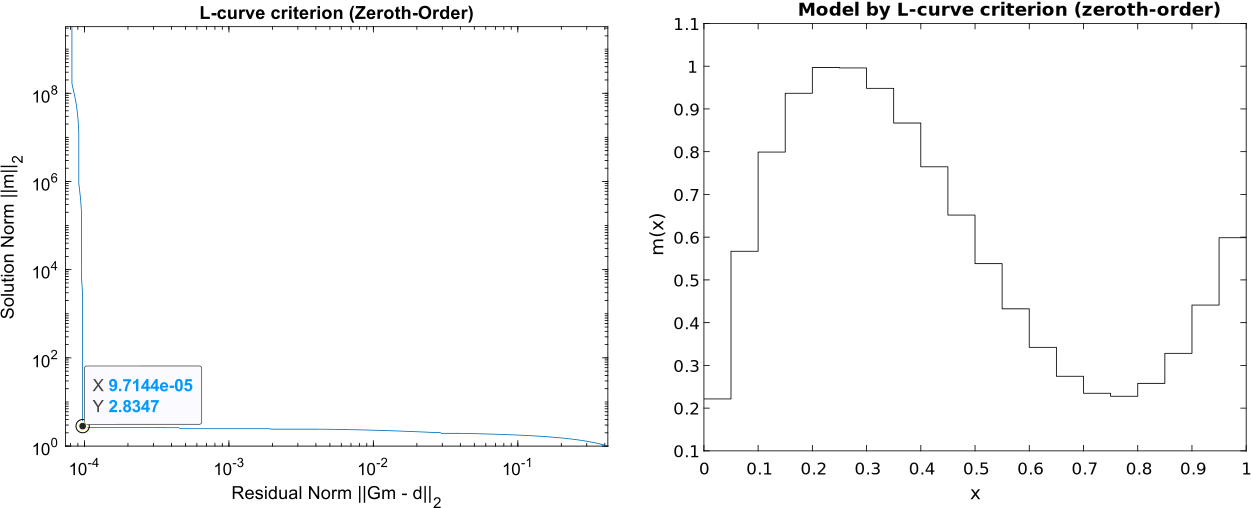
\includegraphics[width=6in, keepaspectratio]{hw5/1.pdf}
    \label{fig:1}
\end{figure}

The discrepancy principle result ($\alpha = 6.7487 \times 10^{-4}$):

\begin{figure}[H]
    \centering
    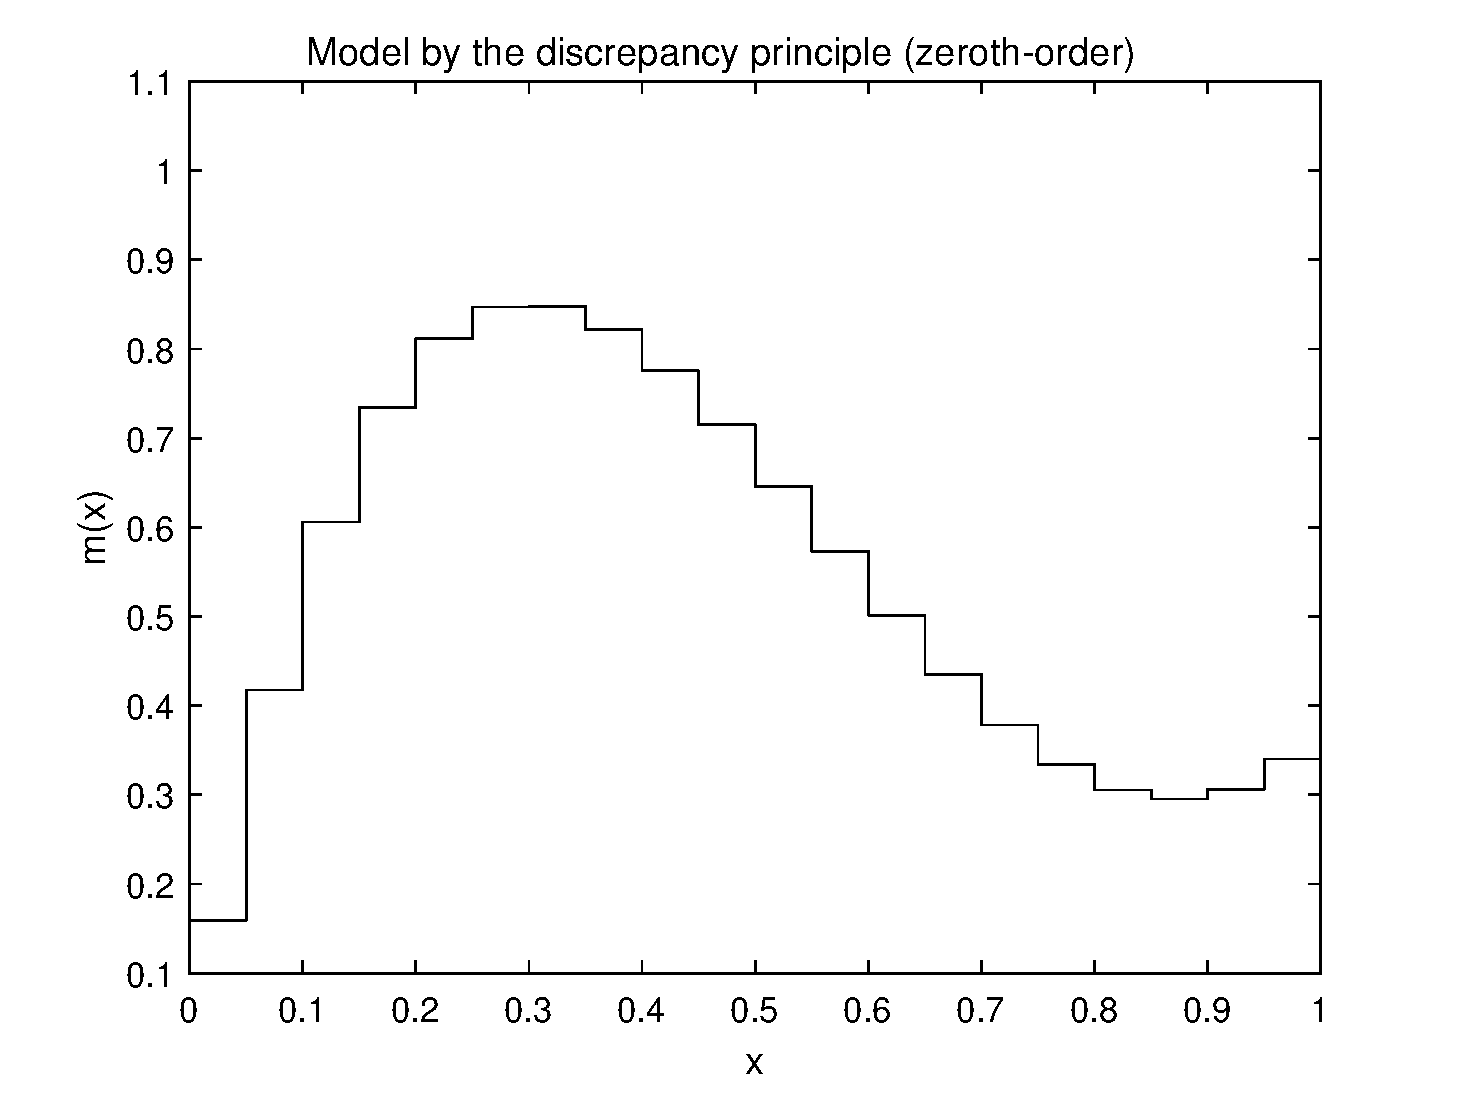
\includegraphics[width=3in, keepaspectratio]{hw5/2.pdf}
    \label{fig:2}
\end{figure}

The GCV result($\alpha = 5.5628 \times 10^{-5}$):

\begin{figure}[H]
    \centering
    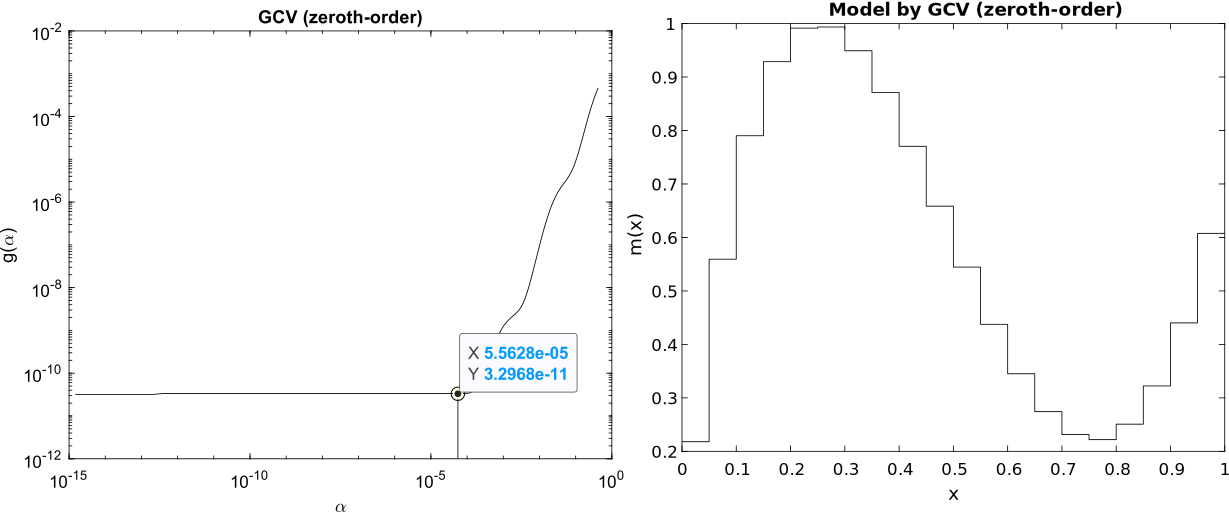
\includegraphics[width=6in, keepaspectratio]{hw5/3.pdf}
    \label{fig:3}
\end{figure}


\part 

Use first-order Tikhonov regularization to solve the problem. Use GCV, the
discrepancy principle, and the L-curve criterion to pick the regularization
parameter.

\solution
The L-curve criterion reslut ($\alpha = 2.277 \times 10^{-4}$):

\begin{figure}[H]
    \centering
    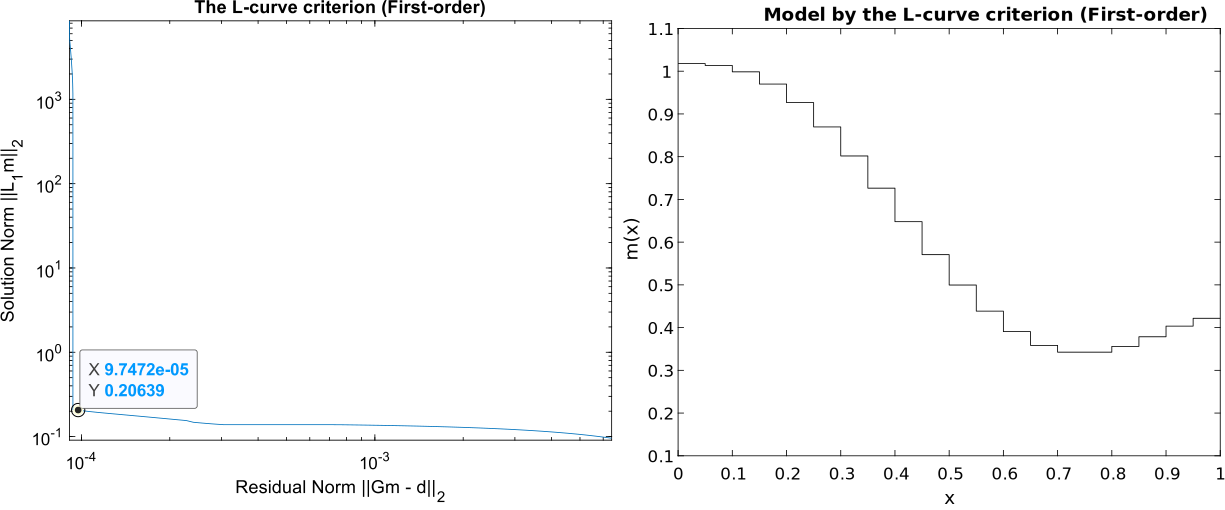
\includegraphics[width=6in, keepaspectratio]{hw5/4.pdf}
    \label{fig:4}
\end{figure}

The discrepancy principle result ($\alpha = 1.68 \times 10^{-2}$):

\begin{figure}[H]
    \centering
    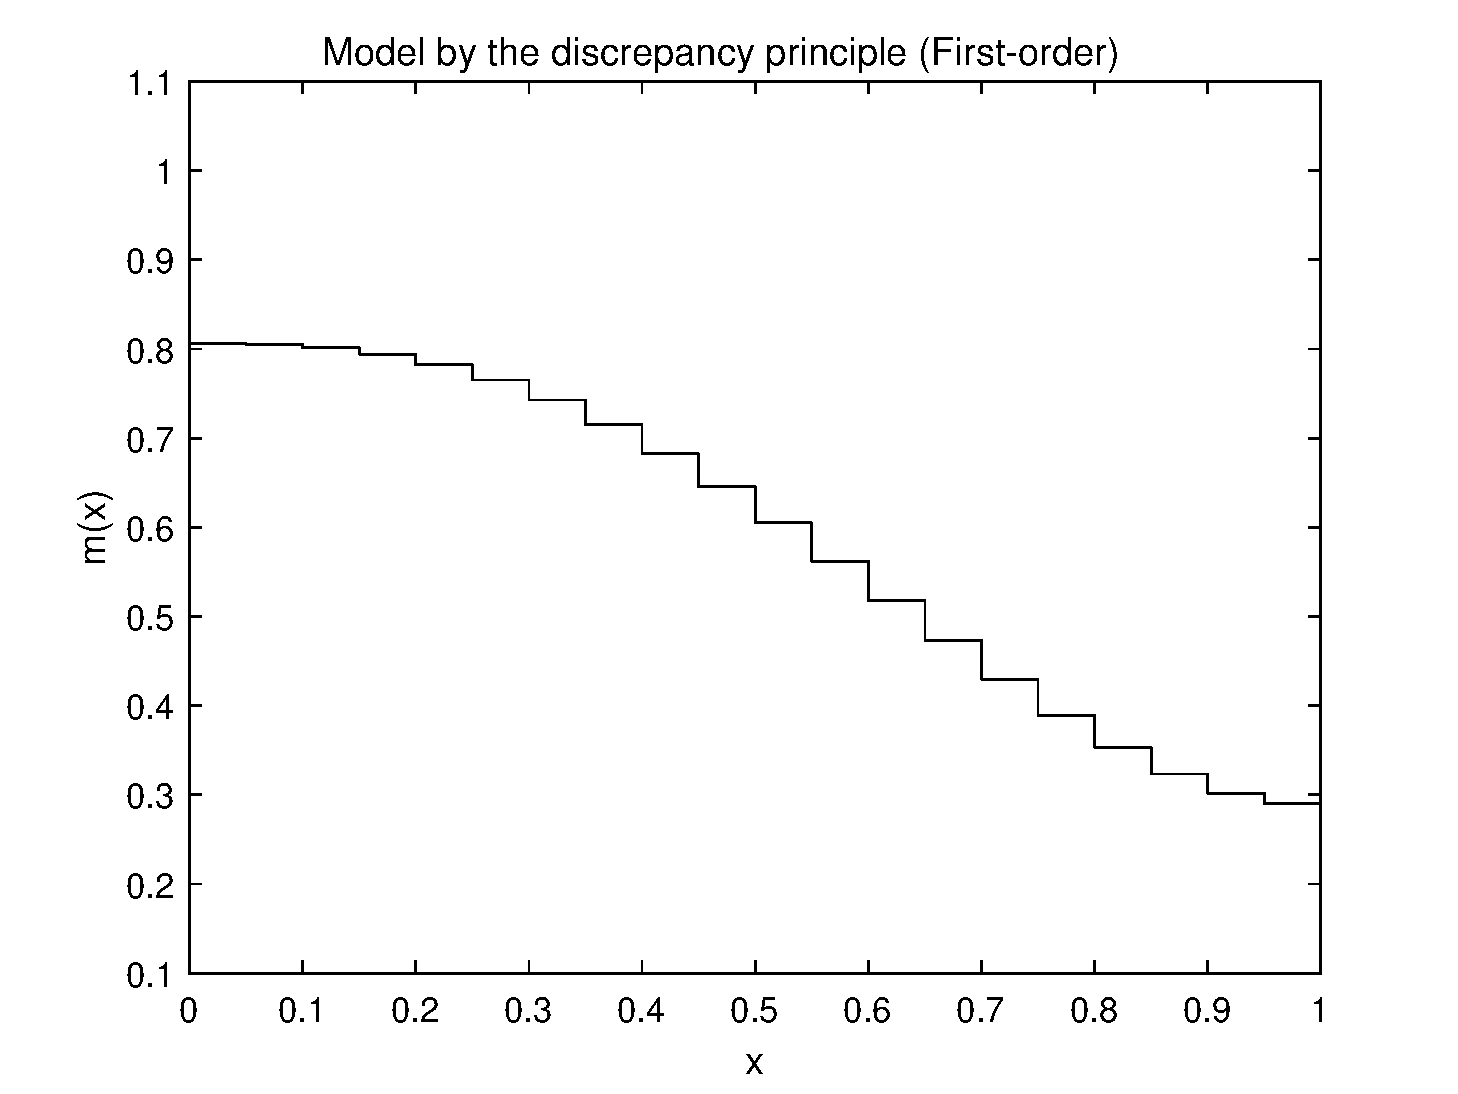
\includegraphics[width=3in, keepaspectratio]{hw5/5.pdf}
    \label{fig:5}
\end{figure}

The GCV result ($\alpha = 6.7487 \times 10^{-4}$):

\begin{figure}[H]
    \centering
    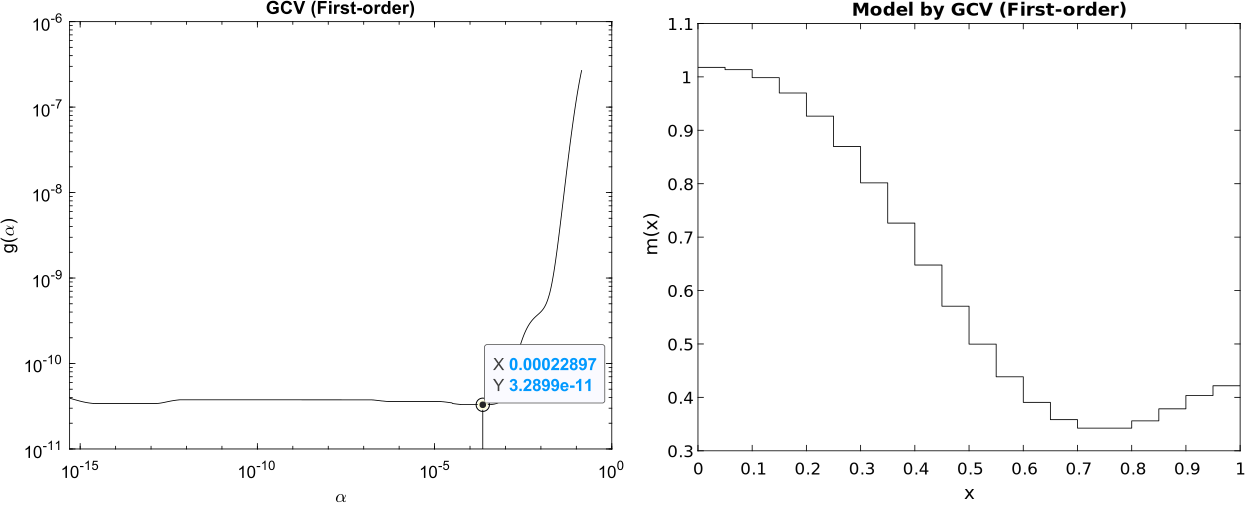
\includegraphics[width=6in, keepaspectratio]{hw5/6.pdf}
    \label{fig:6}
\end{figure}

\end{homeworkProblem}

\begin{homeworkProblem}[3]
Consider the following problem in \textbf{cross-well tomography}. Two vertical wells
are located 1600 m apart. A seismic source is inserted in one well at depths of
50, 150, ... , 1550 m. A string of receivers is inserted in the other well at depths
of 50 m, 150 m, ... , 1550 m. See Figure~\ref{fig:prob}. For each source-receiver pair, a
travel time is recorded, with a measurement standard deviation of 0.5 ms. There are
256 ray paths and 256 corresponding data points. We wish to determine the velocity
structure in the two-dimensional plane between the two wells.

\quad Discretizing the problem into a 16 by 16 grid of 100 meter by 100 meter blocks
gives 256 model parameters. The \textbf{G} matrix and noisy data, \textbf{d}, 
for this problem (assuming straight ray paths) are in the file \textbf{crosswell.mat}. 
The order of parameter indexing from the slowness grid to the model vector is 
row by row (e.g., Example 1.12).

\begin{figure}[H]
    \centering
    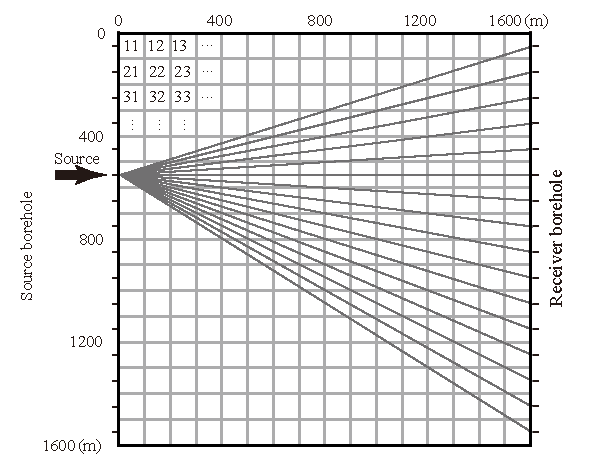
\includegraphics[width=4in, keepaspectratio]{hw5/prob.pdf}
    \caption{Cross-well tomography problem, showing block discretization, 
    block numbering convention, and one set of straight source-receiver ray paths.}
    \label{fig:prob}
\end{figure}

\part 

Use the TSVD to solve this inverse problem using an L-curve. Plot the result.

\solution

\begin{figure}[H]
    \centering
    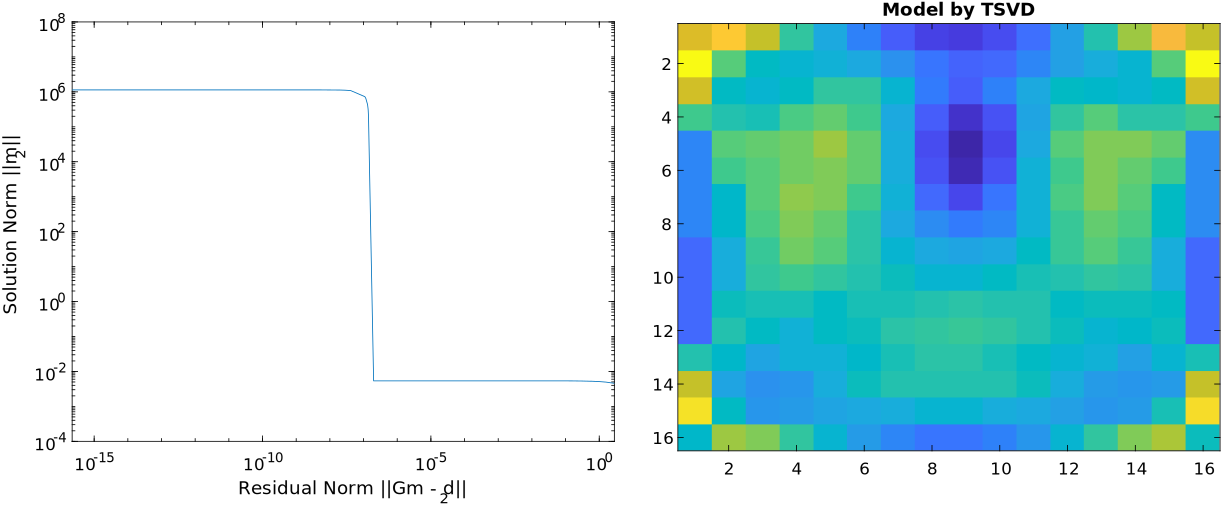
\includegraphics[width=6in, keepaspectratio]{hw5/7.pdf}
    \label{fig:7}
\end{figure}

\part 

Use zeroth-order Tikhonov regularization to solve this problem and plot your
solution. Explain why it is difficult to use the discrepancy principle to select the
regularization parameter. Use the L-curve criterion to select your regularization
parameter. Plot the L-curve as well as your solution.

\solution

Because $\delta = \sqrt{256}\times5\times10^{-4} = 0.008$, it is too large to 
case a poor result by the discrepancy principle. The L-curve criterion's results are 
shown blow.

\begin{figure}[H]
    \centering
    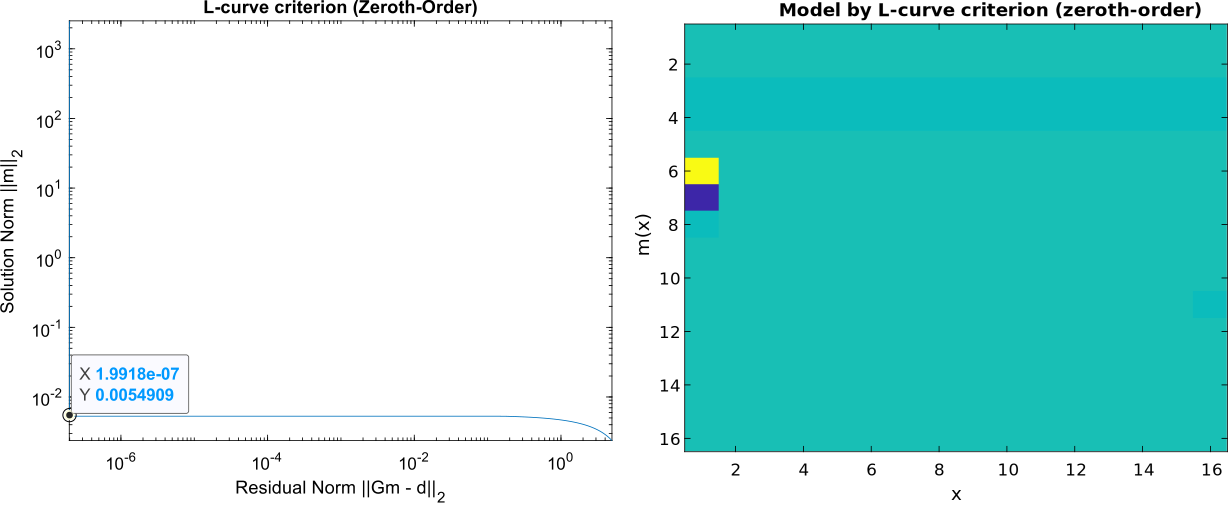
\includegraphics[width=6in, keepaspectratio]{hw5/8.pdf}
    \label{fig:8}
\end{figure}



\part 

Use second-order Tikhonov regularization to solve this problem and plot your
solution. Because this is a two-dimensional problem, you will need to implement
a finite-difference approximation to the Laplacian (second derivative in the
horizontal direction plus the second derivative in the vertical direction) in
the roughening matrix. The \textbf{L} matrix can be generated using the following
\textbf{MATLAB} code:
\begin{lstlisting}[language={matlab}]
L=zeros(14*14,256);
k=1;
for i=2:15,
    for j=2:15,
        M=zeros(16,16);
        M(i,j)=-4;
        M(i,j+1)=1;
        M(i,j-1)=1;
        M(i+1,j)=1;
        M(i-1,j)=1;
        L(k,:)=reshape(M,256,1)';
        k=k+1;
    end
end
\end{lstlisting}

What, if any, problems did you have in using the L-curve criterion on this
problem? Plot the L-curve as well as your solution.

\solution

\begin{figure}[H]
    \centering
    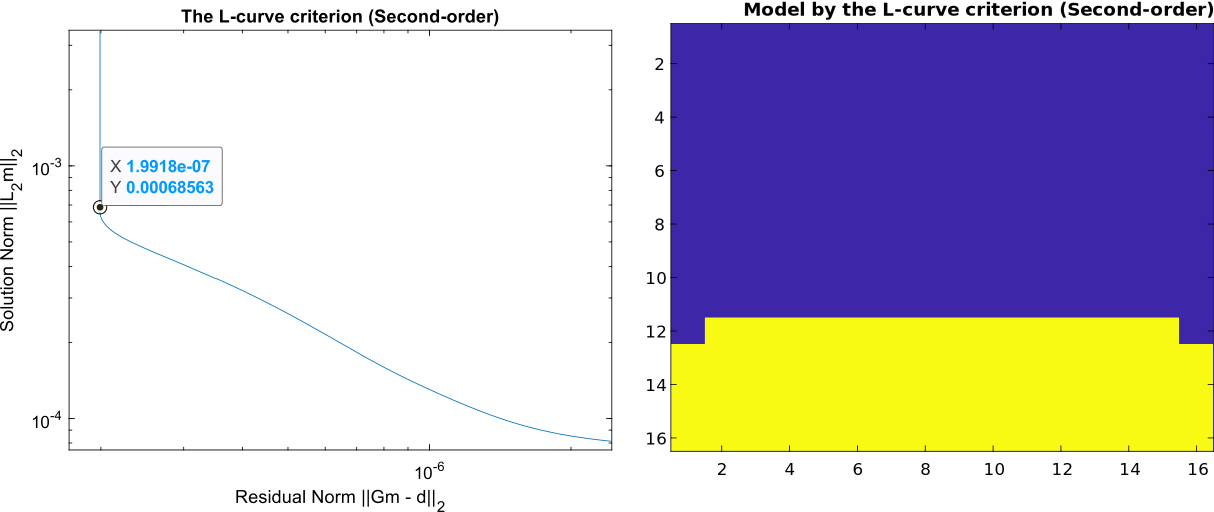
\includegraphics[width=6in, keepaspectratio]{hw5/9.pdf}
    \label{fig:9}
\end{figure}

\part 

Discuss your results. If vertical bands appeared in some of your solutions, can you
explain why?

\solution

It might be decided by resolution matrix.

\end{homeworkProblem}

\begin{homeworkProblem}[5]
In some situations it is appropriate to bias the regularized solution toward a particular
model $\mb{m}_0$. In this case, we would solve
\begin{equation}
    \min \|\mathbf{G m}-\mathbf{d}\|_{2}^{2}+\alpha^{2}\left\|\mathbf{L}
    \left(\mathbf{m}-\mathbf{m}_{0}\right)\right\|_{2}^{2}
\end{equation}
Write this as an ordinary linear least squares problem. What are the normal
equations? Can you find a solution for this problem using the GSVD?

\solution

Refered to the page 95, we can get:

\begin{equation}
    \begin{aligned}
    & \min  \Vert \mt{\mb{G} \\ \alpha \mb{L}}\mb{m} - 
    \mt{\mb{d} \\ \alpha \mb{Lm}_0} \Vert_2^2 \\
    & \text{normal equation} \Rightarrow \\
    & \mt{\mb{G}^T & \alpha \mb{L}^T} \mt{\mb{G} \\ \alpha \mb{L}} 
    \mb{m} = \mt{\mb{G}^T & \alpha \mb{L}^T} \mt{\mb{d} \\ \alpha \mb{Lm}_0} \\
    \Rightarrow & (\mb{G}^T\mb{G} + \alpha^2 \mb{L}^T\mb{L})(\mb{m}-\mb{m_0}) = 
    \mb{G}^T (\mb{d} - \mb{Gm}_0)
    \end{aligned}
\end{equation}

Since, we assume $[UVXAB] = gsvd(G, L)$, so:
\begin{equation}
    \begin{aligned}
    (\mb{A}^T\mb{A} + \alpha^2\mb{B}^T\mb{B})\mb{X} = \mb{A}^T\mb{B}^T(\mb{d}-\mb{Gm}_0) \\
    x_i = \frac{\gamma_i^2}{\gamma_i^2 + \alpha^2} = 
    \frac{\mb{U}_{.i+k}^T(\mb{d}-\mb{Gm}_0)}{\lambda_i} .
    \end{aligned}
\end{equation}

If we set $\mb{KX} = \mb{m}-\mb{m}_0$, we will obtain:
\begin{equation}
    \mb{m} = (\sum_{i=1}^m \frac{\gamma_i^2}{\gamma_i^2 + \alpha^2} 
    \frac{\mb{U}_{.i+k}^T (\mb{d}-\mb{Gm}_0)}{\lambda_i} \mb{K}_{.i} ) + \mb{m}_0
\end{equation}


\end{homeworkProblem}

\end{document}
